\subsection{Anforderungsanalyse mittels Use-Case-Betrachtung}
% TODO: Struktur der Überschriften ändern, diese hat nur einen 
% Unterpunkt und passt thematisch nicht

\subsubsection{Interaktion über Slack}

Es werden folgende Befehle für die Interaktion definiert.

\begin{table}[H]
\centering
\begin{tabular}{l|l}
  Befehl & Bedeutung \\
 \hline
% für vergessliche Leute
 zeige Schicht & zeigt die nächste Schicht für die aufrufende Person an \\
 zeige Schichten & zeigt alle zukünftigen Schichten für die aufrufende Person an \\
 zeige alle Schichten & zeigt einen Schichtplan an, welcher alle Mitglieder enthält \\
 
% jedes Mitglied muss pro Jahr mindestens x mal an die Bar
 zeige Anzahl Schichten & zeigt die geleisteten Schichten für dieses Jahr an \\
 zeige Anzahl alte Schichten & zeigt die geleisteten Sichten für letztes Jahr an \\
 
% zum Anzeigen der Auswahl an welchen man teilnehmen  möchte
 zeige Termine & zeigt alle kommenden Termine $t_i$ an \\
 zeige Veranstaltungen & zeigt alle zukünftigen Veranstaltungen $v_i$ an ($V \subseteq T$) \\
 zeige Sitzungen & zeigt alle zukünftigen Sitzungen $s_i$ an ($S \subseteq T$) \\
 
% für Termin eintragen
 nehme Teil an $t_i$ & trägt den aufrufenden Nutzer als Teilnehmer für $t_i$ ein \\
 nehme nicht Teil an $t_i$ & trägt den aufrufenden Nutzer für $t_i$ aus\\

 % Utilities
 hilf mir & zeigt alle verfügbaren Kommandos an \\
 Danke & bricht die aktuelle Konversation ab
 
 wann ist der nächste termin?
 trag mich ein
 
 
\end{tabular}
\caption{Befehle zur Chatbotinteraktion}
\label{tab:chatbotinteraktion}
\end{table}

Die Befehle in \autoref{tab:chatbotinteraktion} folgen einem vereinfachtem Schema natürlicher Sprache: \texttt{<Prädikat (Imperativ)> <Subjekt>}. Die Struktur der Befehle soll dabei einfach zu merken, auf menschlicher Sprache basierend und auch auf mobilen Geräten mit wenig Tipparbeit verwendbar sein. Bei einem optionalen Einsatz einer Spracherkennung sind auch komplexere Satzkonstruktionen möglich, für den hier zu erfüllenden Zweck genügt das Schema aus \texttt{<Befehl> <Objekt> <Filter>}. Wie in \cite{ZueConversationalinterfacesadvances2000} beschrieben, weicht die Art der Kommunikation von Mensch-zu-Mensch und Mensch-zu-Bot voneinander ab, worauf bei der Definition der Interaktionsbefehle geachtet wurde. Es ist nach Ansicht der Autoren wenig sinnvoll, einen Bot zu entwickeln, der durch den Zugriff auf große Datenmengen den Eindruck von Intelligenz vermittelt, die aber durch ihre Begrenzung dem Nutzer keinen Mehrwert bietet. Der hier entwickelte Bot verfügt bewusst über ein begrenztes Vokabular, so dass er nur die vom Nutzer gewünschten Informationen liefert; die Kenntnis der Befehle obliegt dem Nutzer.

Aus den in \autoref{tab:chatbotinteraktion} definierten Befehlen wurden die Aktivitätsdiagramme \autoref{img:activity-zeige} und \autoref{img:activity-teilnahme} erstellt, um die Reihenfolge der Interaktion besser zu strukturieren.

\begin{figure}[htbp]
    \centering
    \includegraphics[width=\textwidth]{../docs/uml/activity-zeige.png}
    \includegraphics[width=0.9\textwidth]{../docs/uml/activity-zeige2.png}
    \caption{Aktivitätsdiagramme zum Anzeigen von Terminen}
    \label{img:activity-zeige}
\end{figure}

\begin{figure}[htbp]
    \centering
    \includegraphics[width=0.7\textwidth]{../docs/uml/activity-teilnahme.png}
    \caption{Aktivitätsdiagramm zur Teilnahme an Terminen}
    \label{img:activity-teilnahme}
\end{figure}


\subsection{Datenbankschema}

Das Datenbankschema soll laut Anforderung unabhängig von einem spezifischen Chatbot nutzbar sein. Falls ein Chatbot ausgetauscht oder andere Interaktionsmethoden hinzugefügt werden, darf die Datenbank entsprechend keine Abhängigkeiten besitzen. Es wird deshalb ein Datenbankschema angelegt, welches nur die Terminverwaltung abbildet und anschließend eine Erweiterung hinzugefügt, welche die notwendigen Schlüssel auf die verwendete Plattform abbildet.

Die Autoren haben die Struktur der derzeitigen manuellen Terminverwaltung erfasst und daraus ein Schema entworfen. Bei diesem Prozess sind Zusammenhänge und Begriffe festgelegt und erkannt worden, welche sich im Zusammenhang mit den Anforderungen an ein Terminverwaltungssystem in einem Datenbankschema niederschlagen. Nachfolgend werden diese Informationen erläutert.

Jeder Termin hat einen eine Bezeichnung, wie beispielsweise eine Weihnachtsfeier, Sitzung oder ein Afterwork. Diese Bezeichnungen werden Termintypen genannt und können mehr als einmal auftreten, wobei die Bezeichnungen nach deren Festlegung nicht direkt Terminen zugeordnet werden müssen. So kann eine Bezeichnung Weihnachtsfeier eingeführt werden, diese jedoch noch nicht geplant sein.

Weiterhin gibt es Zeitpunkte oder Zeitspannen, zu denen Termine stattfinden. Der Begriff Termin legt jedoch nicht fest, ob es sich um eine Zeitspanne oder einen Zeitpunkt handelt. So kann der Beginn einer Sitzung festgelegt werden, deren Ende jedoch nicht. Eine Andere Sicht auf Termine wäre die planmäßige Dauer eines Afterworks, wobei der Anfang und ein voraussichtliches Ende bekannt sind.

Wenn ein Termin festgelegt wird und dieser häufiger als einmal auftreten kann, ist es möglich, dass auch die Zeitspannen und Zeitpunkte mehr als einmal auftreten. Ein Afterwork beginnt laut den bekannten Informationen immer 19:00 Uhr, wobei zwei Schichten geplant sind, da die Mitglieder nicht über den ganzen Abend Bardienst haben wollen. Die erste Schicht dauert zwei Stunden, endet demnach gegen 21:00 Uhr, während die zweite Schicht 21:00 Uhr beginnt und meist bis 23:00 geht. Der Bardienst der letzten Schicht kann nach eigenem Ermessen festlegen, ob die Bar später schließt oder nicht. Für die Verwaltung ist letzteres jedoch nicht relevant.

Die Mitglieder sollen weiterhin die Möglichkeit haben, sich in diese Schichten einzutragen. Es muss deshalb eine Zuordnung von den Schichten eines Termins und Nutzern geben. 


Um die Anforderungen in einer Datenbank modellieren zu können, wurde ein Schema erstellt, welches diese Abbildet. Die Autoren werden die Entscheidungen hierbei erläutern. Es wurde versucht ein Datenbankschema in der 3. Normalform zu erstellen, um Redundanzen zu vermeiden und Eindeutigkeit zu erreichen. guter grund????????????

Der Termintyp eines Termins wurde in eine extra Tabelle ausgelagert, da dieser Mehrfach auftreten kann und deshalb redundant ist. Ein Termin muss eindeutig identifiziert werden können, weshalb eine ID eingeführt wird. Weiterhin erhält ein Termin ein Datum, welches den Tag des Beginns enthält. Ein Termintyp kann angelegt werden, ohne einem Termin zugeordnet zu sein, jedoch auch beliebig vielen Terminen zugeordnet werden, weshalb die Kardinalität \texttt{1 : 0..*} sein muss.

Schichten erhalten ebenfalls eine eigene Tabelle, da diese sonst redundante Informationen einführen würden. Um eine Schicht mit einem Termin zu verbinden, muss eine Zuordnung erfolgen, weshalb eine Tabelle Terminschicht eingeführt wird. Über diese sind Termine, deren Namen und Schichten eindeutig identifizierbar. Es sollen Schichten angelegt werden können, ohne diese direkt Terminen bzw. der Terminschichttabelle zuweisen zu müssen, jedoch sollen Schichten beliebig vielen Terminen zugeordnet werden können. Die Kardinalität muss deshalb \texttt{1 : 0..*} zwischen Schicht und Terminschicht sein. Da ein Termin mehrere Schichten haben kann, demnach mehrfach in der Terminschichttabelle stehen kann und mindestens eine Zeit bzw. Schicht festgelegt haben muss, ist die Kardinalität zwischen Termin und Terminschicht \texttt{1 : 1..*}.

Nutzer erhalten ebenfalls eine eigene Tabelle mit einer ID. Die Nutzer müssen anschließend zu Terminschichten, d.h. zu eindeutigen Zeitspannen oder Zeitpunkten zugeordnet werden, wodurch eine Zuordnungstabelle Nutzerschicht benötigt wird. Da sich ein Nutzer in mehrere Schichten eintragen kann, jedoch auch keine Schicht belegt haben muss, ist die Kardinalität zwischen Nutzer und Nutzerschicht \texttt{1 : 0..*}. Eine Terminschicht muss keine Zuordnung zu einem Nutzer haben. Dies ist der Fall, wenn sich kein Nutzer für eine Schicht eintragen ließ. Die Kardinalität zwischen Terminschicht und Nutzerschicht ist dementsprechend ebenfalls \texttt{1 : 0..*}.

Die Zuordnung zu den verwendeten Chatplattformen ist nicht Teil der Terminverwaltung, soll jedoch nicht ausgelassen werden, weshalb eine Tabelle \texttt{<Plattform>}nutzer für jede Plattform angelegt werden kann, welche die IDs der Nutzer zu den Namen innerhalb einer Plattform zuordnet. Ein Nutzer einer Plattform ist hierbei immer eindeutig einem internen Nutzer zugeordnet. Ein interner Nutzer muss jedoch nicht Mitglied jeder Plattform sein. Es ist denkbar, dass sich ein Nutzer auf einer bestimmten Plattform mehr als einen Account anlegt und diesen mit dem intern eindeutigen Nutzer verbinden möchte. Dieser Fall soll nicht ausgeschlossen werden, weshalb die Kardinalität zwischen \texttt{<Plattform>}nutzer und Nutzer \texttt{0..* : 1} betragen muss.

Die Umsetzung der vorgestellten Informationen ist in \autoref{img:db-schema} ersichtlich.


% Hier das DB-Schmea rein und eine Fremdschlüsseltabelle für die Slack-Nutzernamen und bla

\begin{figure}[htbp]
    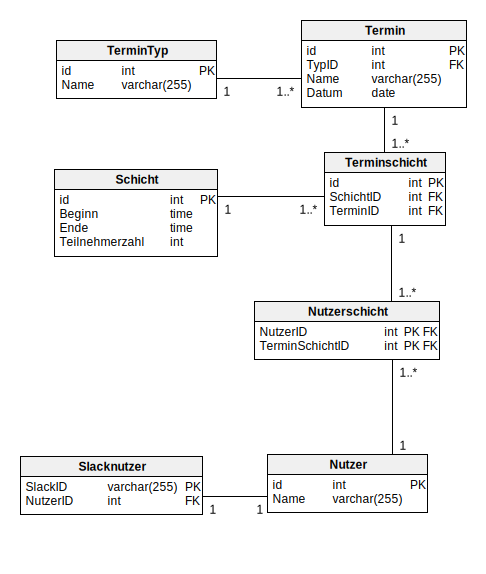
\includegraphics[width=\textwidth]{../docs/uml/Steckerbot-DB.png}
    \caption{Schema der Termin-Datenbank}
    \label{img:db-schema}
\end{figure}


\subsection{Kommunikationsschnittstellen}

Die kommunikation zwischen der Datenbank und dem Chatbot erfolgt auf dem gleichen Host, weshalb keine besonderen Fälle beachtet werden müssen. Der Kommunikationspfad zwischen dem Chatbot und Slack wird jedoch über ein Hochschulnetzwerk durchgeführt. In diesem sind in das Netzwerk des Clubs nur die Ports 80 und 443 freigegeben. Ausgehend ????????????????? doppeltes NAT aber Webseiten ok

Aus diesem Grund muss der Chatbot sich als Client mit Slack verbinden und darf keine Serveranwendung sein, welche ein Polling implementiert.

% vllt Grafik einfügen?


TODO: ERWEITERN
Slack hat eine option globale UIDs zum bot durchzuleiten. nützlich, wenn mehrere Workspaces genutzt werden - ist das der fall? ferdi fragen.
